% !TEX root = ./amsa_main.tex
\section{Coordinate Friendly Operators}\label{sec:cuf}

\subsection{Notation}
For convenience, we do not distinguish \emph{a coordinate} from \emph{a block of coordinates} throughout this paper. We assume our variable $x$ consists of $m$ coordinates: $$x = (x_1, \ldots, x_m) \in\HH := \HH_1 \times \cdots \times \HH_m\quad\mbox{and}\quad x_i\in\HH_i,~ i=1,\ldots,m.$$ For simplicity, we assume that $\HH_1,\ldots,\HH_m$ are finite-dimensional real Hilbert spaces, though most results hold for general Hilbert spaces.
A function maps from $\HH$ to $\RR$, the set of real numbers, and an operator maps from $\HH$ to $\GG$, where the definition of $\GG$ depends on the context. \cut{The operator $\cT$ and those operators in the splitting methods in \S\ref{sec:splitting} map from $\HH$ to $\HH$.}

Our discussion often involves two points $x,x^+\in\HH$ that \emph{differ by one coordinate}: there exists an index $i\in\{1,\ldots,m\}$ and a point $\delta_i\in\HH$ that is supported on $\HH_i$, such that
\beq\label{singleupdate}
x^+ = x+\delta_i.
\eeq
Note that $x^+_j=x_j$ for all $j\not=i$. 
\begin{definition}[number of operations]
We let $\nops{a}{b}$ denote \emph{the number of basic operations} that it takes to compute the quantity $b$ from the  input $a$.
\end{definition}
For example, $\nops{x}{(\cT x)_i}$ denotes the number of operations to compute the $i$th component of $\cT x$ given a general point $x$. We explore the possibility to compute  $(\cT x)_i$ with much fewer operations than what is needed to first compute $\cT x$ and  then take its $i$th component. %Obviously, this number  depends on the structure of $\cT$.   

For a given matrix $A$, let $A_{i,:}$ and $A_{:,j}$ be its $i$th row and $j$th column, respectively. Let $A^\top$ be the transpose of $A$ and $A^\top_{i,:}$ be $(A^\top)_{i,:}$, i.e., the $i$th row of the transpose of $A$. 

\subsection{Single Coordinate Friendly Operators}
This subsection studies a few classes of CF operators and then formally define the CF operator. We motivate the first class through an example.
\begin{example}[least squares]\label{ex:lsq1}
Consider the least squares problem
\begin{equation}
\Min_{x} f(x):=\frac{1}{2} \|A x - b\|^2,\label{lsq}
\end{equation}
where $A \in \RR^{p \times m}$ and $b \in \RR^p$. In this example, assume that $m=\Theta(p)$, namely, $m$ and $p$ are of the same order.  We compare the full update of gradient descent to its coordinate update.\footnote{Although gradient descent is seldom used to solve least squares, it often appears as a part in first-order algorithms for problems involving a least squares term.} 
The full update is referred to as the iteration
$x^{k+1}= \cT x^k $ where $\cT$ is defined as
\begin{equation}
\cT x:=x-\eta\nabla f(x)=x-\eta A^\top Ax + \eta A^\top b.
\end{equation}
Assuming that $ A^\top A$ and $ A^\top b$ are already computed, we have $\nops{x}{\cT x}=O(m^2)$. The coordinate update at the $k$th iteration performs
$$x_{i_k}^{k+1}=\cT_{i_k} x^k =x^k_{i_k}-\eta\nabla_{i_k} f(x^k),$$
and $x_j^{k+1}=x_j^{k},\forall j\neq i_k$, where $i_k$ is some selected coordinate. 

Since for all $i$, $\nabla_i f(x^k)=\left(A^\top (Ax-b)\right)_{i}=(A^\top A)_{i,:}\cdot x-(A^\top b)_{i}$,
we have $\nops{x}{\cT_i x }=O(m)=O(\frac{1}{m}\nops{x}{\cT x})$. Therefore, the coordinate gradient descent is computationally worthy. 
\end{example}
The operator $\cT$ in the above example is a special \emph{Type-I CF} operator.
\begin{definition}[Type-I CF]
For an operator $\cT: \HH\to\HH$, let $\nops{x}{(\cT x)_i}$ be the number of operations for computing the $i$th coordinate of $\cT x$ given $x$ and $\nops{x}{\cT x}$ the number of operations for computing $\cT x$ given $x$. 

We say $\cT$ is \emph{Type-I CF} (denoted as $\cF_1$) if for any $x\in\HH$ and $\forall\, i\in\{1,\ldots,m\}$, it holds
$$\nops{x}{(\cT x)_i}= O\bigg(\frac{1}{m}\nops{x}{\cT x}\bigg).$$
\end{definition}
\begin{example}[least squares II]\label{ex:lsq2}
We can implement the coordinate update in Example \ref{ex:lsq1} in a different manner by maintaining the result $\cT x^k$ in the memory throughout, which works when $m=\Theta(n)$ or $p\gg m$. The full update is unchanged. 
At each iteration, from $\cT x^k$ we immediately obtain $x_{i_k}^{k+1}=(\cT x^k )_{i_k}$ but  need to refresh $\cT x^k$ to $\cT x^{k+1}$.
Since $x^{k+1}$ and $x^k$ only differ by just one coordinate, the refreshing only requires multiplying the $i_k$th column of $A^\top A$ by $x^{k+1}_{i_k}-x^k_{i_k}$, which is much cheaper than multiplying $A^\top A$ by $x^{k+1}$. The work of refreshing takes $O(m)$ operations, which is $O(\frac{1}{m}\nops{x}{\cT (x)})$.
Therefore,
$$\nops{\{ x^k,\cT x^k, x^{k+1}\}}{ \cT x^{k+1}}= O\bigg(\frac{1}{m}\DIFdelbegin  \nops{x^{k+1}}{\cT  x^{k+1}} \bigg).$$
\end{example}
The operator $\cT$ in the above example is a special \emph{Type-II CF} operator.

\begin{definition}[Type-II CF]
An operator $\cT$ is called \emph{Type-II CF} (denoted as $\cF_2$) if, for any $x,i,\delta_i,x^+$ satisfying \eqref{singleupdate}, the following holds
\begin{equation}\label{op-cuf2} \nops{\{ x,\cT x, x^+\}}{ \cT x^+}= O\bigg(\frac{1}{m}\nops{x^+}{\cT x^+}\bigg).
\end{equation}
\end{definition}
Sometimes, maintaining certain quantities other than $\cT x$ can also make the coordinate update computationally worthy.
\begin{example}[least squares III]\label{ex:lsq3}
For the case $p\ll m$, i.e., the system $Ax=b$ is highly underdetermined, we should avoid pre-computing $A^\top A$ because multiplying $A$ and then $A^\top$ is cheaper. Therefore, we change the implementations of both the full and coordinate updates in Example \ref{ex:lsq1}. In particular, the full update
$$x^{k+1}=\cT x^k =x^k-\eta\nabla f(x^k)=x^k-\eta A^\top (Ax^k-b),$$
pre-multiplies $x^k$ by $A$ and then $A^\top$. Hence, 
$\nops{x^k}{\cT(x^k)}=O(mp)$.

We change the coordinate update to maintain the intermediate quantity $Ax^k$. The coordinate update computes 
$$(\cT x^k)_{i_k}=x^k_{i_k}-\eta (A^\top Ax^k-A^\top b)_{i_k},$$
by pre-multiplying $Ax^k$ by $A^{\top}_{i_k,:}$ and refreshing $Ax^k$ to $Ax^{k+1}$ by adding $(x^{k+1}_{i_k}-x^k_{i_k}) A_{:,i_k}$ to $A x^k$. Both steps take $O(p)$ operations, so
\begin{displaymath}{\nops{\{x^k,Ax^k\}}{\{x^{k+1},Ax^{k+1}\}}=O(p)=O\left(\frac{1}{m}\nops{x^k}{\cT x^k}\right)}.\end{displaymath}
\end{example}
Combining Type-I and Type-II CF operators with the last example, we arrive at the following definition:

\begin{definition}[CF operator]
 We say that an operator $\cT:\HH\to\HH$ is \emph{CF} if, for any $x,i,\delta_i,x^+$ satisfying \eqref{singleupdate}, the following holds 
%given any $x\in\HH$ and an arbitrary $i\in\{1,\ldots,m\}$, the coordinate update from $x$ to $x^+$ where $x^+_i = (\cT x)_i$ and $x_{j}^+=x_{j}$ for $j\not=i$, satisfies
\begin{equation}\label{op-cuf} \nops{\{x,\cM(x)\}}{\{x^+,\cM(x^+)\}}= O\bigg(\frac{1}{m}\nops{x}{\cT x}\bigg),
\end{equation}
where $\cM(x)$ is some quantity maintained in the memory to facilitate each coordinate update and refreshed to $\cM(x^+)$. $\cM(x)$ can be empty, i.e., besides $x$, there is no other varying quantity maintained.
\end{definition}

\cut{\begin{definition}[CF operator]
We say that an operator $\cT:\HH\to\GG$ is \emph{coordinate-update (CU) friendly} if for a generic $\eta\in \HH$, $\forall i\in\{1,\ldots,\dim\GG\}$ and $\forall j\in\{1,\ldots,\dim\HH\}$:
\begin{equation}\label{op-cuf}\nops{\{x, \eta_j, \cT x\} }{(\cT (x+\eta_j e_j))_i}\le O\bigg(\frac{1}{\dim \GG}\nops{\{x,\eta,\cT x\}}{\cT (x+\eta)}\bigg).
\end{equation}
(Maintaining quantities other than $x$ and $\cT x$ in  memory is allowed.)
The \emph{set} of CF operators is denoted by  $\cF$. \commzp{$e_j$ is not defined.}
\end{definition}
}

The left-hand side of \eqref{op-cuf} measures the cost of performing one coordinate update (including the cost of updating $\cM(x)$ to $\cM(x^+)$)  while the right-hand side measures the average per-coordinate cost of updating all the coordinates together. When~\eqref{op-cuf} holds, $\cT$ is amenable to coordinate updates.

\cut{\begin{example}Consider for $a,x\in\RR^m$, $$f(x):=\frac{1}{2}\big(\max(0,1-\beta a^\top x)\big)^2,$$ which is the squared hinge loss function. Consider the operator 
\beq\label{qhlossT}
\cT x:=\nabla f(x)=-\beta \max(0,1-\beta a^\top x) a.
\eeq
Let us maintain $\cM(x)=a^\top x$. For arbitrary $x$ and $i$,  let $$x^+_i:=(\cT x)_i=-\beta \max(0,1-\beta a^\top x) a_i$$ and $x^+_j:=x_j,\,\forall j\neq i$. Then, computing $x^+_i$ from $x$ and $a^\top x$ takes $O(1)$ (as $a^\top x$ is maintained), and computing $a^\top x^+$ from $x^+_i-x_i$ and $a^\top x$ costs $O(1)$. Formally, we have
\begin{align*}
&\nops{\{x,a^\top x\}}{\{x^+,a^\top x^+\}}\\
=&\nops{\{x,a^\top x\}}{x^+}+\nops{\{a^\top x,x^+_i-x_i\}}{a^\top x^+}\\
=&O(1)+O(1)=O(1).
\end{align*} 
On the other hand, $\nops{x}{\cT x}=O(m)$. Therefore,~the inequality \eqref{op-cuf} holds, and $\cT$ defined in~\eqref{qhlossT} is CF.
\end{example}
}
\cut{Next, we specify two sub-types of CF operators. They have  stronger properties that are useful when composing with other operators.
\begin{definition} Consider an operator $\cT: \HH\to\HH$.
\begin{itemize}
Let $\mathfrak{M}(x\to (\cT x)_i)$ be the number of operations of computing the $i$-th coordinate of $\cT x$ given $x$ and $\mathfrak{M}(x\to\cT x)$ the number for computing $\cT x$ given $x$.

\item $\cT$ is \emph{Type-I CF} (denoted as $\cF_1$) if for any $x\in\HH$ and $\forall\, i\in\{1,\ldots,m\}$, it holds
$$\nops{x}{(\cT x)_i}= O\bigg(\frac{1}{m}\nops{x}{\cT x}\bigg).$$

%\item Type-II CF ($\cF_2$): an operator $\cT:\HH\to\GG$ is in $\cF_2$ if, for any $x\in\HH$,  $c\in\RR$, it holds that, $\forall i=1,\ldots,\dim\GG$ and $\forall j=1,\ldots,\dim\HH$:  $$\nops{\{x,\cT x,c\}}{(\cT (x+c e_j))_i}\le O\left(\frac{1}{\dim\GG}\nops{\{x,\cT x,c\}}{\cT (x+ce_j)}\right).$$

\item $\cT$ is \emph{Type-II CF} (denoted as $\cF_2$) if, for any $x,i,\delta_i,x^+$ satisfying \eqref{singleupdate}, the following holds: 
\begin{equation}\label{op-cuf2} \nops{\{ x,\cT x, x^+\}}{\cT x^+}= O\bigg(\frac{1}{m}\nops{x^+}{\cT x^+}\bigg)
\end{equation}

\end{itemize}
\end{definition}}
%\begin{remark}
By definition, a Type-I CF operator $\cT$ is CF without maintaining any quantity, i.e., $\cM(x)=\emptyset$. 

A Type-II CF operator $\cT$ satisfies \eqref{op-cuf} with $\cM(x)= \cT x$, so it is also CF. Indeed, given any $x$ and $i$, we can compute $x^+$ by immediately letting $x^+_i=(\cT x)_i$ (at $O(1)$ cost) and keeping $x^+_{j}=x_{j},\,\forall j\neq i$; then, by \eqref{op-cuf2}, we update $\cT x$ to $\cT x^+$ at a low cost. Formally, letting $\cM(x)= \cT x$, %Assume $x$ is updated from $x^-$ and they differ only at the $j$th coordinate, i.e., $x_j=(\cT x^-)_j$ and $x_{j'}=x^-_{j'},\,\forall j'\neq j$. Then we have
\begin{align*}
&\nops{\{x, \cM(x)\}}{\{x^+,\cM(x^+)\}}\\
\le &\nops{\{x, \cT x\}}{x^+} + \nops{\{x, \cT x, x^+\}}{\cT x^+}\\
\overset{\eqref{op-cuf2}}= & O(1) +O\bigg(\frac{1}{m}\nops{x^+}{\cT x^+}\bigg)\\
= & O\bigg(\frac{1}{m}\nops{x}{\cT x}\bigg).
\end{align*} %Type-I CF operators include all separable operators (see Definition \ref{def:sep-op} and Examples \ref{exp:diagmat} through \ref{exp:proj-box} below), and Type-II CF operators include the affine mapping $\cT x=Ax+b$ as a special case.

\cut{\begin{example}[Matrix-vector multiplication]\label{ex:mtx}
Let $A \in \RR^{m \times m}$ be dense, and $A_{i,:},A_{:,i}$ be the $i$th row and the $i$th column of $A$, respectively. Let $b\in\RR^{m}$. Consider $$\cT x:= A x + b,$$ 
and   $x,i,\delta_i,x^+$ satisfying \eqref{singleupdate} for $\HH=\RR^m$. Clearly, $\nops{x}{\cT x}=O(m^2)$.

\begin{enumerate}
\item Since $(\cT x)_i=A_{i,:} x+b_i$ takes $(m+1)$ operations, we have $\nops{x}{(\cT x)_i}=m+1=O(\frac{1}{m}\nops{x}{\cT x})$, so $\cT$ is Type-I CF.
\item Let us maintain $\cM(x)=\cT x$. Since $\cT x^+=\cT x+(x^+_i-x_i)A_{:,i} $ takes $2m+1$ operations, we have $\nops{\{ x,\cT x, x^+\}}{\cT x^+}=O(\frac{1}{m}\nops{x}{\cT x})$. Therefore, $\cT$ is  Type-II CU friendly (by maintaining $\cT x$).
\end{enumerate}
Whether maintaining $\cT x$ or nor will  make significant difference when $\cT$ pre-composes or post-composes another operator.
\end{example}
}
\cut{ let $a_i$ be the $i$th row of $A$. We have $\nops{x}{\cT(x)}=\nops{x}{Ax+b}=m^2+m$, and  $\nops{x}{(\cT }$}
\DIFdelbegin %DIFDELCMD < 

%DIFDELCMD < %%%
In general, the set of CF operators is much larger than the union of Type-I and Type-II CF operators.
%\end{remark}
%{\color{red} we have to declare what one coordinate means here (it can be one block of coordinate whenever it is used together}

%CF operators, as the name suggests, let one compute coordinate updates at little overhead.
Another important subclass of CF operators are operators $\cT:\HH\to\HH$ where   $(\cT x)_i$ only depends on one, or a few, entries out of $x_1,\ldots,x_m$.\cut{, obviously $(\cT x)_i$ is relatively easy to compute. Therefore, they belong to $\cF$.} Based on how many input coordinates they depend on, we partition them into three subclasses.
 \DIFdelbegin %DIFDELCMD < 

%DIFDELCMD < %%%
\DIFdelend \begin{definition}[Separable operator]\label{def:sep-op} Consider $\mathfrak{T}:=\{\cT:\HH\to\HH\}$. We have the partition $\mathfrak{T}=\cC_1\cup\cC_2\cup\cC_3$, where
\cut{We divide the operators into three categories base on the dependency of other coordinates when updating one coordinate.}
\begin{itemize}
\item \emph{separable operators:} $\cT\in\cC_1$ if, for any index $i$, there exists $\cT_i: \HH_i \rightarrow \HH_i$ such that $(\cT x)_i = \cT_i x_i$, that is,   $(\cT x)_i$ only depends on $x_i$.
\item \emph{nearly-separable operators:} $\cT\in \cC_2$ if, for any index $i$, there exists $\cT_i$ and index set $I_i$ such that $(\cT x)_i = \cT_i(\{x_j\}_{j\in I_i})$ with $|I_i| \ll m$, that is, each $(\cT x)_i$ depends on a few  coordinates of $x$.
\item \emph{non-separable operators:} $\cC_3:=\mathfrak{T}\setminus(\cC_1\cup \cC_2)$. If $\cT\in\cC_3$, there exists some  $i$ such that $(\cT x)_i$ depends on many coordinates of $x$.
\end{itemize}
\end{definition}

\cut{For operators in $\cC_1$, the evaluation of $(\cT x)_i$ only involves coordinates $x_i$ and small operator $\cT_i$.  Thus, all the coordinates and the $\cT_i$s are independent with each other, and this is ideal case for coordinate update. For operators in $\cC_2$, the evaluation of $(\cT x)_i$ needs knowledge of some components of $x$.}

Throughout the paper, we assume the coordinate update of a (nearly-) separable operator costs roughly the same for all coordinates. Under this assumption, separable operators are both Type-I CF and Type-II CF, and nearly-separable operators are Type-I CF.\footnote{\label{note1}Not all nearly-separable operators are Type-II CF. Indeed, consider a sparse matrix $A\in \RR^{m\times m}$ whose  non-zero entries are only located  in the last column. Let $\cT x=Ax$ and $x^+=x+\delta_m$. As $x^+$ and $x$ differ by the last entry, $\cT x^+=\cT x+(x^+_m-x_m)A_{:,m}$ takes $m$ operations. Therefore, we have $\nops{\{x,\cT x,x^+\}}{\cT  x^+}=O(m)$. Since $\cT x^+=x^+_mA_{:,m}$ takes $m$ operations, we also have $\nops{x^+}{\cT x^+}=O(m)$. Therefore,~\eqref{op-cuf2} is violated, and there is no benefit  from maintaining $\cT x$.}  %DIF > There are non-separable  CF operators, e.g., Example \ref{ex:lsq1}, \ref{ex:lsq2}, \ref{ex:lsq3}. 
%For example, with a (dense) matrix $A\in\RR^{m\times m}$ and vector $b\in\RR^{m}$, the operator $\cT:x\mapsto A x+b$ is non-separable yet CF. Indeed, let $a_i$ be the $i$th row of $A$. We have $\nops{x}{\cT(x)}=\nops{x}{Ax+b}=m^2+m$, and  $\nops{x}{(\cT x)_i}=\nops{x}{a_i^\top x+b_i}=m+1$, which is much smaller. 

\cut{There are CF operators that are not Type-I . For example, let $f(x)=\sum_{i=1}^m \log [1+\exp(-b_i a_i^\top x)]$. The gradient operator $\nabla f$ is not Type-I CF, but it is CF by caching $a_i^\top x,\, \forall i$.}


\cut{Next, we defined \emph{easy-to-update} operators. While they are not CF,  $\cT x$ can  be easily updated after the input $x$ is changed on one or a few of its coordinates. Therefore, by maintaining $\cT x$  in memory, they are also amenable to coordinate update computing. %For an update-to-update operator $\cT$, \cut{because $\cT x$ can be cheaply updated, }it is important to maintain  $\cT x$  in memory.

\begin{definition}[Easy-to-update]
We say an operator $\cT:\HH\to\GG$ is  \emph{easy-to-update} if, for any $x\in \HH$ and  $c\in\RR$, it holds that $\forall i=1,\ldots,\dim\HH$: $$\nops{\{x,\cT x, c\}}{\cT(x+c e_i)}\le O\left(\frac{1}{\dim\HH}\big(\nops{\{x, c\}}{x+c e_i} +\nops{x+c e_i}{\cT (x+c e_i)}\big)\right).$$
The \emph{set} of {easy-to-update} operators is denoted by $\cE$.
\end{definition}

\cut{A (nearly-) separable operator $\cT$ (i.e., in $\cC_1\cup\cC_2$) is easy-to-coordinate-update if $\cT x$ is maintained in the memory. }


In coordinate-update algorithms, easy-to-update operators \emph{can be treated as} a subclass of CF operators. Seemingly, an easy-to-update operator is not CF since it is not necessarily cheaper to compute $(\cT x)_i$ than the entire $\cT  x$. However, computing the entire $\cT  x$ and changing the entire $x$ add a significantly higher cost to \emph{the next iteration} than computing just $(\cT x)_i$, changing just $x_i$, and taking advantage of the easy-to-update property.
}

%Summarizing this subsection, coordinate update algorithms shall apply CF operators, which include separable, nearly-separable,  linear, as well as easy-to-update operators. 
\cut{
Finally, we define \emph{cheap} and \emph{easy-to-maintain} operators from $\HH$ to $\GG$ that arise in operator compositions.
\begin{definition}[Cheap operator] In an operator composition $\cT=\cT_1 \circ\cdots \circ \cT_p$, an operator $\cT_i:\HH\to\GG$ is cheap if $\nops{x}{\cT_i x}$ is less than or equal to the number of remaining coordinate-update operations, in order of magnitude.
\end{definition}
\begin{definition}[Easy-to-maintain operator]
%If $\cT$ maps from $\HH$ to a different space $\GG$ and it satisfies \eqref{op-cuf2}, we call it 
In an operator composition $\cT=\cT_1 \circ\cdots \circ \cT_p$, an operator $\cT_i:\HH\to\GG$ is \emph{easy-to-maintain} if, for any $x,i,\delta_i,x^+$ satisfying \eqref{singleupdate}, $\nops{\{ x,\cT x, x^+\}}{\cT x^+}$ is less than or equal to the number of remaining coordinate-update operations, in order of magnitude, \emph{or} belongs to $O(\frac{1}{\dim \GG}\nops{x^+}{\cT x^+})$.

The set of  easy-to-maintain operators is denoted by $\cE$. %We call an operator $\cT: \HH\to\GG$ \emph{easy-to-update} if it  and denote the set of these operators as $\cE$.  
\end{definition}
%Easy-to-update operators are used in maintaining quantities.
}

\cut{
\begin{definition}[Easy-to-update]
We say an operator $\cT:\HH\to\GG$ is  \emph{easy-to-update} if, for any $x$ and  $\delta=\sum_{i\in\II}\eta_i e_i$ of arbitrary coefficient $\eta_i\in\RR$ and a small index set $\II$ ($|\II|\ll m$), it holds that  $$\nops{\{x,\cT x,(\eta_i)_{i\in\II}\}}{\cT(\tilde x)}\ll\nops{\{x,(\eta_i)_{i\in\II}\}}{\tilde x} +\nops{\tilde x}{\cT\tilde x},$$
where $\tilde x=x+\delta$. The \emph{set} of {easy-to-update} operators is denoted by $\cE$.
\end{definition}
}

 \cut{When one or a few coordinates of $x$ are changed, giving the new point $\tilde x$, we compute $(\cT \tilde x)_i$ by refreshing $\cT x$ at a low cost. It would be much more expensive to first form $\tilde x$ and then compute $T\tilde x$.}
%In this section, we would like to introduce some properties for single operators.

%
%\begin{definition}[CF]
%One operator is called CF if there is no additional cost for updating all the coordinates one by one independently comparing to updating all the coordinates together. There are mainly three types of CF operators:
%\begin{itemize}
%\item $\cC_1$: updating one coordinate depends ONLY on this coordinate.
%\item $\cC_2$: updating one coordinate depends on SOME coordinates.
%\item $\cC_3$: updating one coordinate depends on ALL coordinates.
%\end{itemize}
%\end{definition}
%\begin{remark}
%We do not consider the cache of computing here. When we consider the derivative of $f(x)$, we consider the each component to be totally unrelated.
%\end{remark}
%\begin{definition}[Block CF]
%One operator is called Block CF if there is no addition cost for updating all the blocks of coordinates one by one independently comparing to updating all the coordinates together. There are mainly three types of Block CF maps:
%\begin{itemize}
%\item $\cB_1$: updating one block of coordinates depends ONLY on this block of coordinates.
%\item $\cB_2$: updating one block of coordinates depends on SOME blocks of coordinates.
%\item $\cB_3$: updating one block of coordinates depends on ALL blocks of coordinates.
%\end{itemize}
%\end{definition}
%\begin{remark}Note that Block CF is just a block version of CF. For Block CF operators, updating all the coordinates one by one independently may introduce additional cost comparing to updating all the coordinates.
%\end{remark}

%To illustrate the properties, we introduce several examples for all the cases.
%\subsection{BC-friendly with property $\cC_1$}
%Assume $\HH = \HH_1 \times \cdots \times \HH_m$, where $m > 0 $ is the number of coordinates. If $\cT: \HH \rightarrow \HH$ satisfies the following
%\begin{align}
%(\cT x)_i = \cT_ix_i, \quad i=1,\cdots,m
%\end{align}
%%$$\cT = \begin{bmatrix}\cT_1 & & \\ & \ddots& \\ & & \cT_m\end{bmatrix},$$
%where $\cT_i: \HH_i \rightarrow \HH_i$, then $\cT$ is CF with $\cC_1$. We denote $\cT$ as $\cT=\cT_{1}\times\cdots\times \cT_{m}$. Thus, computing $\cU_i \circ \cT x$ takes no extra effort, since
%$$(\cU_i \circ \cT) x = (\cT x)_i = \cT_i x_i.$$
%The computation only involves a coordinates $x_i$ and a small operator $\cT_i$.  It would be embarrassingly parallelization, since the coordinates and the $\cT_i$s are independent with each other, and the computation can be carried out without any communication.
\subsection{Examples of CF Operators}\label{sec:exp-cuf}
In this subsection, we give  examples of CF operators arising in different areas including linear algebra, optimization, and machine learning.
\begin{example}[(block) diagonal matrix]\label{exp:diagmat}
Consider the diagonal matrix
$$A = \begin{bmatrix}a_{1,1} & ~ & 0 \\  & \ddots&  \\ 0& ~& ~a_{m,m}\end{bmatrix}\in\RR^{m\times m}.$$
Clearly $\cT:x\mapsto Ax$ is separable.
\end{example}
\begin{example}[gradient and proximal maps of a separable function]
Consider a \emph{separable} function
$$f(x) = \sum_{i=1}^m f_i(x_i).$$
Then, both $\nabla f$ and $\prox_{\gamma f}$ are separable, in particular,
$$(\nabla f(x))_i = \nabla f_i (x_i) \quad \mbox{and}\quad (\prox_{\gamma f}(x))_i= \prox_{\gamma f_i} (x_i).$$\cut{$$\nabla f(x) = \begin{bmatrix} \nabla f_1 (x_1) \\ \vdots \\ \nabla f_m(x_m) \end{bmatrix} \quad \mbox{and}\quad \prox_{\gamma f}(x) = \begin{bmatrix}  \prox_{\gamma f_1} (x_1) \\ \vdots \\  \prox_{\gamma f_m}(x_m) \end{bmatrix}.$$}
Here, $\prox_{\gamma f} (x)$ ( $\gamma >0$) is the \emph{proximal operator} that we  define in Appendix~\ref{sec:op-concept}. %returns the minimizer $y^*$ of the function $f(x) + \frac{1}{2\gamma } \|x - y\|^2$. The minimizer exists and is unique when $f$ is a closed proper convex function.
% $$\prox_{\gamma f} (x): = \argmin_{y \in \HH} f(x) + \frac{1}{2\gamma } \|x - y\|^2,$$
% for which we assume unique minimizer (true if $f$ is closed proper convex).
\end{example}

\begin{example}[projection to box constraints]\label{exp:proj-box}
%\commwy{Please move this example to below $\cC_1$. Use the box constraint example instead of $\ell_\infty$ ball since the latter is a special example. Also, please add a proposition that $\cC_1\cup\cC_2\subset\cE$, which is obvious.}
Consider the ``box" set $B:=\{x:a_i\leq x_i\leq b_i,~i=1,\ldots,m\}\subset\RR^m$. Then, the projection operator $\prj_{B}$ is separable. Indeed,
$$\big(\prj_{B}(x)\big)_i=\max(b_i,\,\min(a_i,\, x_i)).$$
%\begin{equation}
%\big(\prj_{B}(x)\big)_i =
%\left\{
%\begin{array}{ll}
%b_i &\text{ if }  x_i \in [b_i, +\infty) \\
%a_i &\text{ if } x_i \in (-\infty, a_i] \\
% x_i &\text{ if } x_i \in [a_i, b_i].
%\end{array}
%\right.
%\end{equation}
\end{example}


\begin{example}[sparse matrices] If every row of the matrix $A\in\RR^{m\times m}$ is sparse,   $\cT :x\mapsto Ax$ is nearly-separable.
%$$A = \begin{bmatrix}A_{11} & A_{12} & \\ A_{21}& A_{22} & \ddots \\ & \ddots & \ddots & A_{m-1,m}\\&  & A_{m,m-1} & A_{m,m}\end{bmatrix},$$
%is a sparse supported map.

Examples of sparse matrices arise from various finite difference schemes for differential equations, problems defined on sparse graphs. When most pairs of a set of random variables  are conditionally independent, their inverse covariance matrix is sparse.
\end{example}

\begin{example}[sum of sparsely supported functions]
Let $E$ be a class of index sets and every $e\in E$ be a small subset of $\{1, ..., m\}$, $|e|\ll m$. In addition $\#\{e:i\in e\}\ll \#\{e\}$ for all $i\in\{1,\ldots,m\}$.
Let $x_e:=(x_i)_{i\in e}$, and  
$$f(x) = \sum_{e \in E} f_e (x_e).$$ 
The gradient map $\nabla f$ is nearly-separable.


An application of this example arises in wireless communication over  a graph of $m$ nodes. Let each $x_i$ be the spectrum assignment to node $i$, each $e$ be a neighborhood of nodes,  and each   $f_e$ be a utility function. The input of $f_e$ is $x_e$ since the utility depends on the spectra assignments in the neighborhood.

In machine learning, if each observation only involves a few features, then each function of the optimization objective will depend on a  small number of components of $x$. This is the case when graphical models are used~\cite{rue2005gaussian,bengio2006label}. \cut{The gradient of $f(x)$ will also only depend on a few coordinates of $x$. \commwy{could you be specific in the machine learning example?}}
\end{example}

\cut{ % have been moved
\begin{example}[matrix-vector multiplication]\label{mtxexam}
With a (dense) matrix $A\in\RR^{m\times m}$, the operator $\cT:x\mapsto A x$ is non-separable yet CF. Indeed, let $a_i$ be the $i$th row of $A$. Then, we can compare $\nops{x}{\cT(x)}=\nops{x}{Ax}=m^2$, and  $\nops{x}{(\cT x)_i}=\nops{x}{a_i^\top  x}=m$ is much smaller.
%Observe that the complexity of $\cS_i \circ (\cT x)$ is $O(m n)$, however, the complexity for evaluating $\cT x$ is $O(n^2)$. We can choose $m \ll n$, then the affine map $\cT$ is BC-friendly.
%The extra cost we pay for parallelization is that $x$ needs to be read $n/m$ times instead of once compared to the serial implementation.
\end{example}
\begin{example}[affine transformation preserves $\cC_1$]
Let $\cT\in\cC_1$, $b \in \HH$. Then $\cT':x\mapsto\cT x + b$ belongs to  $\cC_1$.
\end{example}
}
\cut{\begin{example}[projection to the Euclidean ball]\label{ex:projball}
Let $B_2=\{x\in\RR^m:\|x\|_2\leq r\}$ and $$\cT x:=\prj_{B_2}(x).$$ By definition, %$\cT(x)=\argmin_y \{\|y-x\|_2:\|y\|_2\le r\}$
%\begin{equation}
$\cT(x) =\xi x,~\mbox{where}~\xi=\min\left\{1,\frac{r}{\|x\|_2}\right\}.$
%\end{equation}
Since $\cT x$ depends on all the entries of $x$,  $\cT$ is non-separable.

Nonetheless, the norm map $\cT':x\mapsto \|x\|_2$ is easy-to-maintain. Indeed, given $x$, we can maintain $\cT'(x)=\|x\|_2$. If $x_i$ is updated,  letting $e_i$ be the $i$th standard basis and writing $\bar{x}=x+\eta e_i$, it follows $\|\bar{x}\|_2=\sqrt{\|x\|_2^2+2\eta x_i+\eta^2}$. Therefore,   $\nops{\{x,\|x\|_2,\eta\}}{\|\bar{x}\|_2}=O(1)$ while $\nops{\bar{x}}{\|\bar{x}\|_2}=O(m)$.

\end{example}
}


%{\color{red}These two examples should be moved back}


\cut{\begin{example}[$\cC_2 + \cC_2= \cC_3$]
Let $A_1,A_2\in\RR^{m\times m}$ be sparse matrices. If $A_1+A_2$ is a dense matrix, then $\cT x= Ax=A_1x+A_2x$ belongs to $\cC_3$ though $\cT_1 x= A_1x$ and $\cT_2=A_2x$ both belong to $\cC_2$.
\end{example}
}


%\begin{example}[Linear combination of maps]
%The linear combination of block separable maps with any other BC-friendly maps is also BC-friendly. For example, $I - \gamma \, \nabla f$ is BC-friendly if $\nabla f$ is BC-friendly.
%\end{example}


%\subsection{BC-friendly with property $\cC_2$}
%\begin{definition}[Sparsely supported map]
%Let $I_i$ be a subset of $\{1, ..., m\}$. Consider $\cT: \HH \rightarrow \HH$ that satisfies
%\begin{equation}
%(\cT x)_i = \cT_i(\{x_j\}_{j\in I_i}).
%\end{equation}
%That is evaluating $(\cT x)_i$ only requires knowledge of those components of $x_j$ for $j \in I_i$. If the maximum cardinality $\max_{i} |I_i| \leq c$ and $c \ll m$, then $\cT$ is said to be \emph{sparsely supported}.
%\end{definition}
%%Since for all $i$, evaluating $(\cT x)_i$ only requires a few coordinates of $x$, hence it is significantly easier than computing $\cT x$. As a consequence, sparsely supported maps are BC-friendly.
%
%
\cut{
Based on the categories of an operator and the examples, we know that all operators in $\cC_1$ are CF, operators in $\cC_2$ with $c\ll m$ is also CF. However, some operator in $\cC_3$ are CF, while others are not. There are other ways to determine whether a combination of several operators is CF or not. }

\cut{\begin{remark}
If the complexity of evaluating $\cT_2 x$ is smaller or equals to the complexity of evaluating $\cT_{1,i} x$, then whether the operators $\cT_1+\cT_2$ and $\cT_1\circ\cT_2$ is CF or not depends on whether $\cT_2$ is CF or not.
\end{remark}}

%{\color{red} If $\cT = \cT_1 \circ \cT_2$, easy-to-update also means the complexity of evaluating $\cT_2 \, x$ is smaller or equals to the complexity of evaluating $\cT_{1, i} \, x$. }


%
%
%\subsection{Easy to compute}
%A function $r$ is \emph{proximal friendly} if the following problem  {\color{blue} is not difficult, (or say has closed form representation.)}
%\begin{equation}
%\prox_r(x) = \argmin_{y} r(y) + \frac{1}{2} \|x - y\|^2.
%\end{equation}
%As we have shown before, if $r(x)$ is block separable, then the $\prox_r$ is also block separable. Examples of such include $\ell_1$ norm, indicate function of box constraints $\{x ~|~ a \leq x \leq b\}$, and the $\ell_{2,1}$ norm. Some other non separable examples but easy to evaluate their proximal map include indicate function of $\ell_2$ ball, $\ell_1$ ball, and indicate function of the probability simplex $\{x~|~ \sum_{i=1}^n x_i = 1, x_i \geq 0\}$. The proximal maps correspond to the projection of the sets.
%


%
%\subsection{Easy-to-update maps}
%[NEED TO REFINE THE DEFINITION] An operator $\cT: \HH \rightarrow \HH$ is easy-to-update, if
%$$O(\cT (x + \sum_{i \in \II} \eta_i e_i )) \ll O (\cT \, y), \forall y$$
%where $|\II| \ll m$.

%{\color{red} If $\cT = \cT_1 \circ \cT_2$, easy-to-update also means the complexity of evaluating $\cT_2 \, x$ is smaller or equals to the complexity of evaluating $\cT_{1, i} \, x$. }

%Following the above example, we define the \emph{easy-to-update} operator, where caching is allowed.

\cut{When we apply coordinate update algorithms, we may choose to store some intermediate variables which are easy to update after some coordinates are updated.}

\cut{
\begin{definition} Let $\mathfrak{M}[x\to \cT(x)]$ denote the number of  operations of computing $\cT(x)$ given $x$. Let $\mathfrak{M}[y\to \tilde y]$ denote the number of  operations of computing $\tilde y$ in place given  $y$.
\end{definition}}

\cut{
\begin{remark}By  definition, a separable operator is easy to update (and no quantity needs to be maintained), but not all nearly-separable operators easy to update. For example, consider a sparse matrix $A\in R^{m\times m}$ where all of its non-zero entries are in the last column. Let $\cT x=Ax$ and, given a point $x$ nd $\tilde x=x+\eta_me_m$, compute $(T(x+\eta_me_m))_m$. We have $\nops{\{x,\cT x,\eta_m\}}{\cT \tilde x}=O(m)$ and $\nops{\{x,\eta_m\}}{\tilde x} +\nops{\tilde x}{\cT(\tilde x)}=O(1)+O(m)=O(m)$. There is not benefit  from maintaining $\cT x$.
\end{remark}
}
\begin{example}[square hinge loss function]\label{ex:qhloss}
Consider for $a,x\in\RR^m$, $$f(x):=\frac{1}{2}\big(\max(0,1-\beta a^\top x)\big)^2,$$ which is the squared hinge loss function. Consider the operator 
\beq\label{qhlossT}
\cT x:=\nabla f(x)=-\beta \max(0,1-\beta a^\top x) a.
\eeq
Let us maintain $\cM(x)=a^\top x$. For arbitrary $x$ and $i$,  let $$x^+_i:=(\cT x)_i=-\beta \max(0,1-\beta a^\top x) a_i$$ and $x^+_j:=x_j,\,\forall j\neq i$. Then, computing $x^+_i$ from $x$ and $a^\top x$ takes $O(1)$ (as $a^\top x$ is maintained), and computing $a^\top x^+$ from $x^+_i-x_i$ and $a^\top x$ costs $O(1)$. Formally, we have
\begin{align*}
&\nops{\{x,a^\top x\}}{\{x^+,a^\top x^+\}}\\
=&\nops{\{x,a^\top x\}}{x^+}+\nops{\{a^\top x,x^+_i-x_i\}}{a^\top x^+}\\
=&O(1)+O(1)=O(1).
\end{align*} 
On the other hand, $\nops{x}{\cT x}=O(m)$. Therefore,~\eqref{op-cuf} holds, and $\cT$ defined in~\eqref{qhlossT} is CF.
\end{example}


\cut{\rev{\subsection{Compare Full Update with Coordinate Update}\label{lsqexperiment}
In this subsection, we compare the efficiency of four different coordinate update schemes (cyclic, cyclic permutation, random, and greedy with Gauss-Southwell rule) with the full gradient descent method for solving the least square problem 
$$\Min_{x} \frac{1}{2} \|A x - b\|^2,$$
where $A \in \RR^{p \times m}$ and $b \in \RR^p$. We solve the above problem with the following update scheme
$$x^{k+1} = x^k - \eta_k A^{\top}(A x^k - b),$$
where $\eta_k$ is the step size. This test uses three datasets, which are summarized in Table \ref{tab:ls-data}.  
\begin{table}[!hbtp]
\centering
 \begin{tabular}{lrrrr}
  \toprule
     & $p$  & $m$ & $A$ & $b$\\
   \midrule
   Dataset I & 1000 & 1000 & \texttt{diag([1:m])} & \texttt{ones(m, 1)} \\
   Dataset II & 1000 & 500 & \texttt{randn(m, n)} & \texttt{ones(m, 1)} \\
   Dataset III & 1000 & 500 & \texttt{rand(m, n)} & \texttt{ones(m, 1)} \\
   \bottomrule
\end{tabular}
 \caption{Three datasets for the least square problem\label{tab:ls-data}}
\end{table}

For both full gradient descent method, the step size $\eta$ is set to $\frac{2}{\|A\|_2^2}$. For the four coordinate update methods, if coordinate $i$ is selected, then $\eta_k$ is set to $\frac{1}{(A^{\top}A)_{ii}}$. Since all of the methods have same per epoch complexity, so we measure and compare the per epoch progress in terms of objective error. Figure \ref{fig:ls_a} shows that for Dataset I, both cyclic update, cyclic permutation, and greedy update converge to the optimal solution with one epoch. Random coordinate update converges to the optimal solution after $8$ epochs. However, due to the small step size ($\eta_k = 10^{-6}$), the gradient descent algorithm converges very slowly. For the other two datasets, we observe that greedy coordinate update converges faster than the other methods, and random coordinate update and cyclic shuffle coordinate update give consistent better performance than the full gradient descent algorithm. 
\begin{figure}[!htbp] \centering
    \begin{subfigure}[b]{0.3\linewidth}
        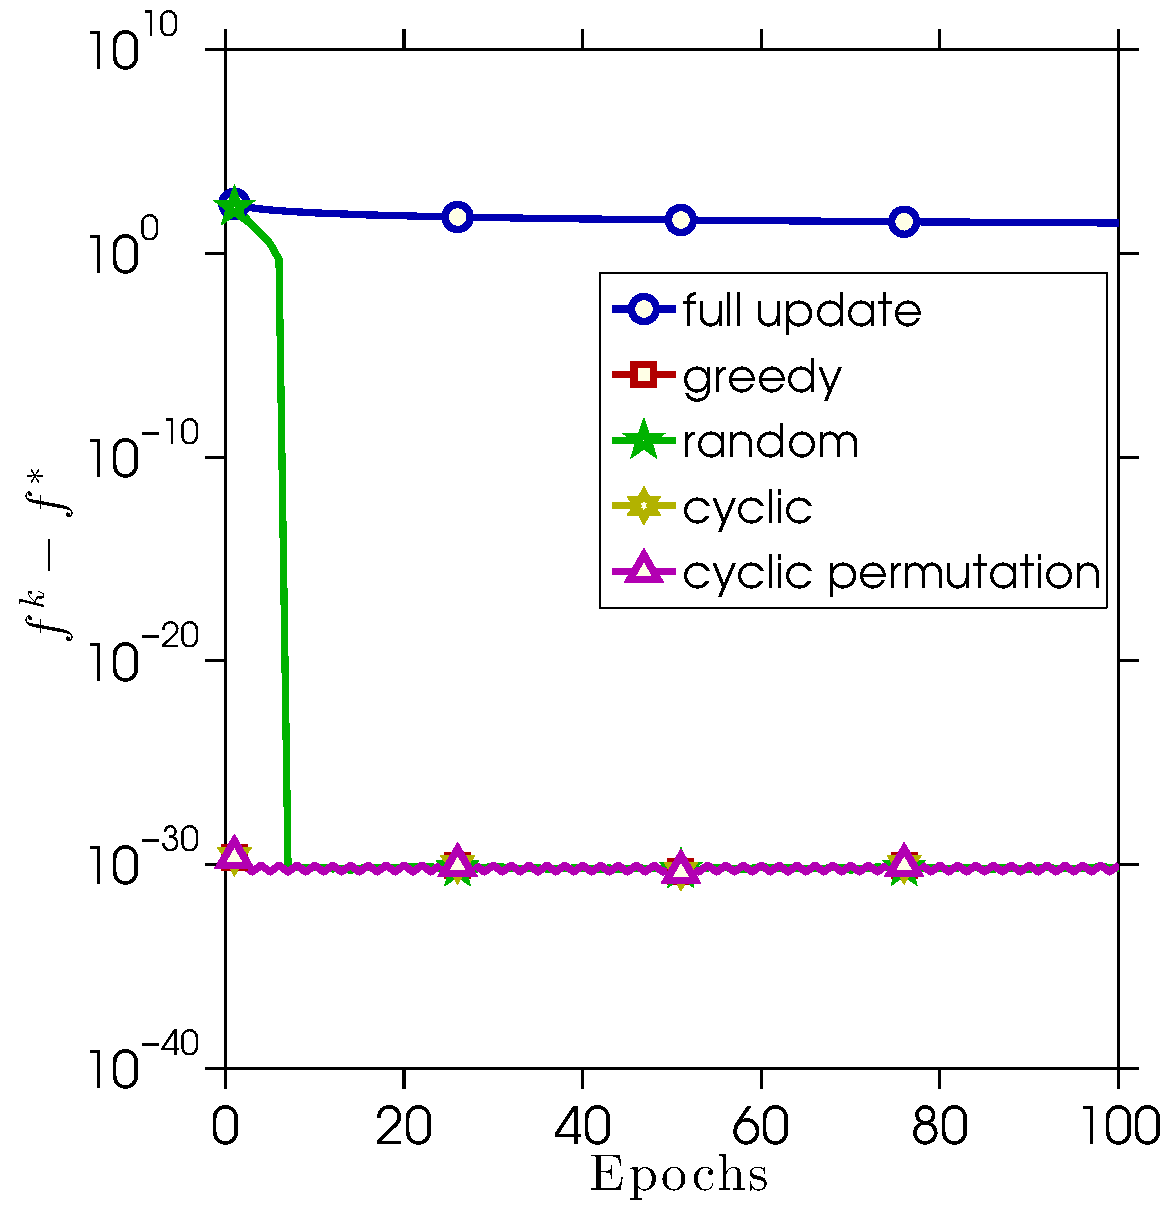
\includegraphics[width=40mm]{./figs/diag_matrix_cropped.pdf}
        \caption{Dataset I}
        \label{fig:ls_a}
    \end{subfigure} %
    \quad
    \begin{subfigure}[b]{0.3\linewidth}
        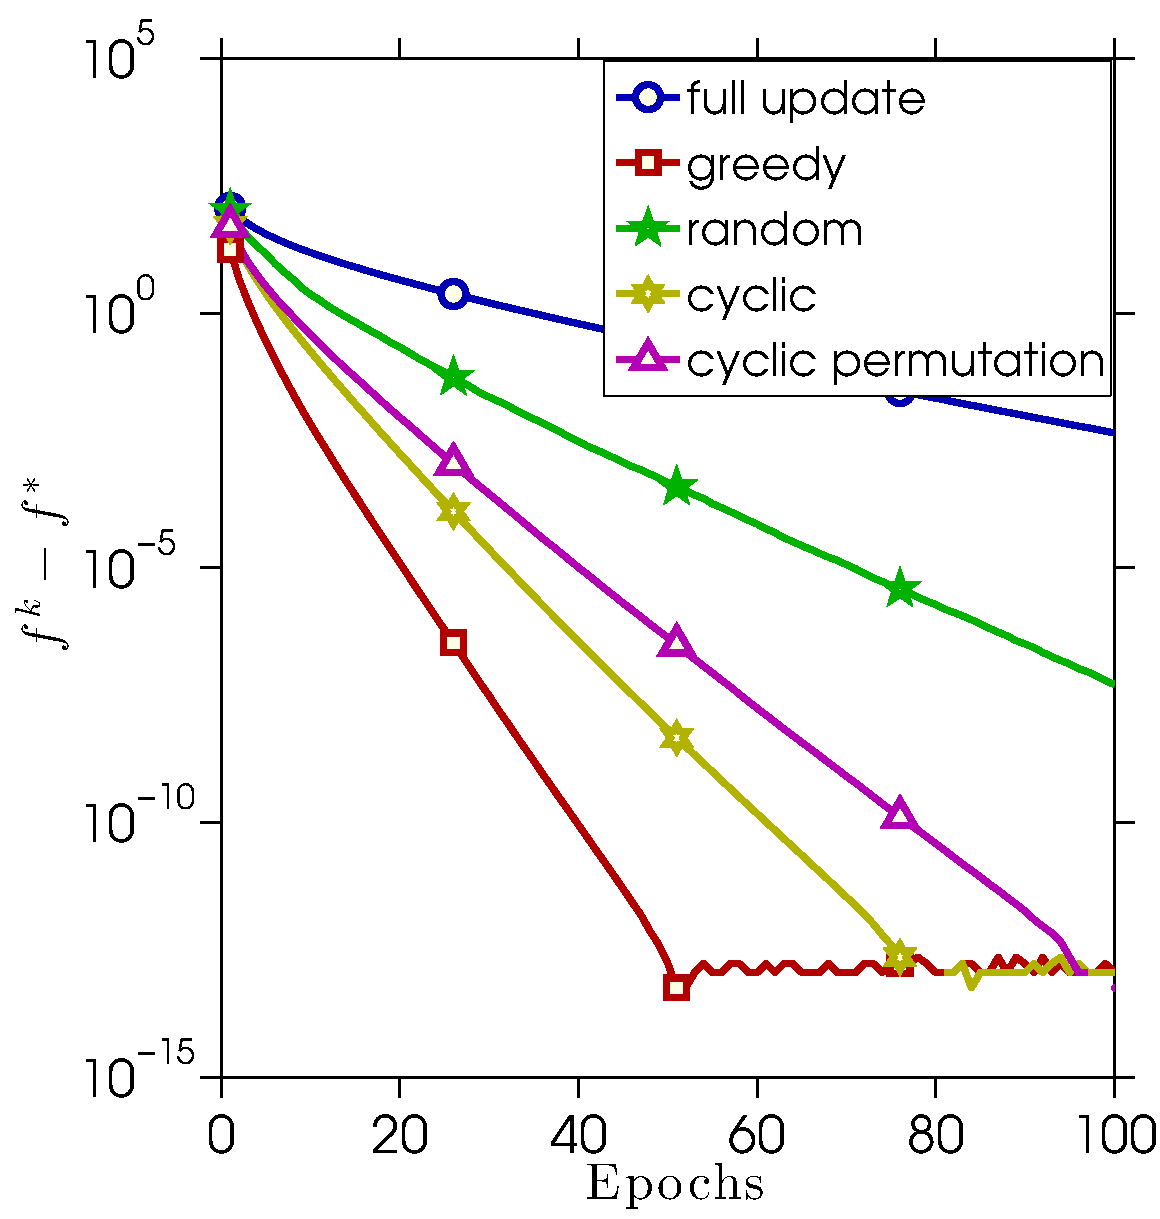
\includegraphics[width=40mm]{./figs/randn_matrix_cropped.pdf}
        \caption{Dataset II}
        \label{fig:ls_b}
    \end{subfigure} %
    \quad
    \begin{subfigure}[b]{0.3\linewidth}
        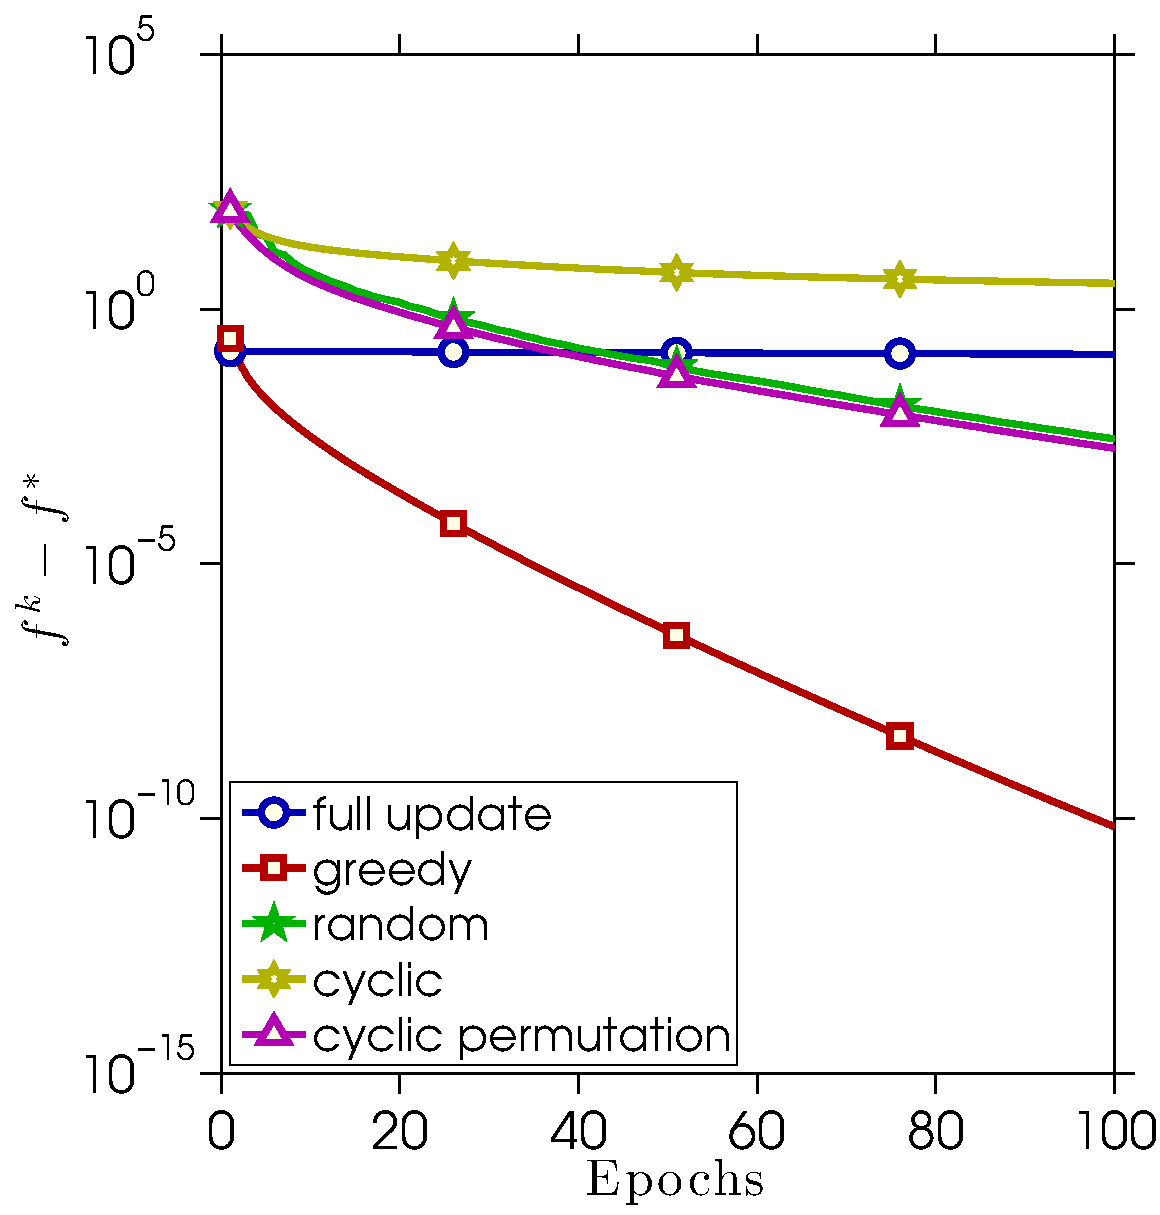
\includegraphics[width=40mm]{./figs/rand_matrix_cropped.pdf}
        \caption{Dataset III}
        \label{fig:ls_c}
    \end{subfigure} %
    \caption{Compare the convergence of four different coordinate update algorithms with full gradient descent algorithm.}
    \label{fig:3s_results}
\end{figure}
}
}

\cut{
\begin{example}[scalar map pre-composing affine function]\label{exp:log-grad} Let $a_j\in \RR^m, b_j\in \RR$ and $\phi_j:\RR\to \RR$ be differentiable functions, $j=1,\ldots,p$. Let $$f(x)=\sum_{j=1}^p \phi_j(a_j^\top x +b_j).$$ Assume that evaluating $\phi'_j$ costs $O(1)$ for all $j$. Then, $\nabla f$ is CF (by maintaining $a_j^\top x+b_j,\,\forall j$), but it is neither Type-I nor Type-II CF if $A=[a_1,\ldots,a_p]^\top$ is dense. Indeed, let $$\cT_1 y:=A^\top y,\quad \cT_2 y := \Diag(\phi_1'(y_1),\ldots,\phi_p'(y_p)), \quad \cT_3 x := Ax+b.$$ Then $\nabla f(x)= \cT_1\circ\cT_2\circ\cT_3 x$. For any $x$ and $i\in\{1,\ldots,m\}$, let $x^+_i=\nabla_i f(x)$ and $x^+_j=x_j,\forall j\neq i$, and let $\cM(x)=\cT_3 x$. We can first compute $\cT_2\circ\cT_3 x$ from $\cT_3 x$ for $O(p)$ operations, then compute $\nabla_i f(x)$ and thus $x^+$ from $\{x, \cT_2\circ\cT_3 x\}$ for $O(p)$, and finally update the maintained $\cT_3 x$ to $\cT_3 x^+$ from $\{x, x^+,\cT_3 x\}$ for another $O(p)$. Formally,
\begin{align*}
&\nops{\{x,\cT_3 x\}}{\{x^+, \cT_3x^+\}}\cr
=& \nops{\cT_3x}{\cT_2\circ\cT_3 x}+\nops {\{x,\cT_2\circ\cT_3 x\}}{x^+}+\nops{\{x,\cT_3 x, x^+\}}{\{\cT_3x^+\}}\cr
=& O(p) + O(p) +O(p)=O(p).\nonumber
\end{align*}
On the other hand, $\nops{x}{\nabla f(x)}=O(pm)$. Therefore
$\nabla f= \cT_1\circ\cT_2\circ\cT_3$ is CF. 

Once $p=m$, $\cT_1,\cT_2,\cT_3$ all map from $\RR^m$ to $\RR^m$. Then, it is easy to check that $\cT_1$ is Type-I CF, $\cT_2$ is separable, and $\cT_3$ is Type-II CF. The last one is crucial since not maintaining $\cT_3 x$ would disqualify $\cT$ from CF. Indeed, to obtain $(\cT x)_i$, we must multiple $A_i^\top$ to all the entries of $\cT_2\circ\cT_3 x$, which in turn needs all the entries of $\cT_3 x$, computing which from scratch costs $O(pm)\gg O(p)$.

There are some  rules to preserve Type-I and Type-II CU-friendliness. For example, $\cT_1\circ \cT_2$ is still Type-I CF, and $\cT_2\circ\cT_3$ is still CF but there are counter examples where  $\cT_2\circ\cT_3$  can be neither Type-I or Type-II CF in general. Such properties are important for developing efficient coordinate update algorithms for complicated problems; see the next section.
\end{example}
}
